\subsection{Primary use case: longitudinal HT-29 screening}

The central use case for BARCS is a continuous predictor observed at more than
two values.  We therefore begin with the HT-29 time course of
\citet{tzelepis2016dropout}, the longitudinal dataset used to evaluate
Chronos \citep{dempster2021chronos}.  It contains a pDNA measurement and HT-29
guide counts at days 7, 10, 13, 16, 19, 22, and 25.
The three sequencing columns at each late day were summed before analysis.
This distinction is important for the requested $t$ inference: three assays of
one harvested population increase read depth but are not three independent
biological units and therefore must not add residual degrees of freedom.
Following the Chronos preprocessing, guides with fewer than 30 pDNA reads were
removed, leaving 86,882 guides targeting 17,995 genes.

The BARCS and official MAGeCK-MLE 0.5.9.5 fits received the same
eight-column count matrix and the same numeric design, with an intercept and
$d_i/25$.  This is a direct continuous-time comparison.  We also downloaded
the all-seven-time-point Chronos joint result and the deposited per-endpoint
MAGeCK and BAGEL2 results from the Chronos Figshare record
\citep{chronosfigshare2021}.  As in the Chronos paper, the latter two were
combined by taking each gene's median effect over the seven separate endpoint
runs.

For an external biological target, core essential genes are positives and
HT-29 genes with DepMap 20Q2 expression below 0.5 are negatives, matching the
deposited Chronos analysis.  All methods were
restricted to the same 1,080 essential and 5,774 unexpressed genes.
Normalized null-median difference (NNMD) is the essential-gene median minus
the unexpressed-gene mean, divided by mean absolute deviation of the
unexpressed effects; more negative values indicate stronger separation.
``False positives'' counts unexpressed genes in the lowest 15\% of all
evaluated effects, following the deposited Chronos analysis.

\begin{table}[ht]
\centering
\caption{Longitudinal HT-29 control-gene benchmark.  PR AUC is the area under
the precision--recall curve; Recall$_{90}$ is the maximum recall at least
90\% precision.  Higher AUROC, PR AUC, and Recall$_{90}$ are better; more
negative NNMD and fewer unexpressed false positives are better.  The best
value in each column is shown in bold and in its method color; row swatches
use the same colors as Figure~\ref{fig:chronos}.}
\label{tab:chronos}
\small
\setlength{\tabcolsep}{4pt}
\begin{tabular}{lrrrrr}
\toprule
Method & AUROC & PR AUC & NNMD & Recall$_{90}$ & FP$_{15\%}$\\
\midrule
\methodswatch{barcsblue} BARCS time & 0.9786 & 0.9494 & $-12.35$ &
  \textcolor{barcsblue}{\textbf{0.9037}} &
  \textcolor{barcsblue}{\textbf{74}}\\
\methodswatch{mageckorange} Official MAGeCK time &
  \textcolor{mageckorange}{\textbf{0.9789}} &
  \textcolor{mageckorange}{\textbf{0.9534}} & $-13.14$ & 0.8972 & 76\\
\methodswatch{chronosgreen} Chronos joint & 0.9747 & 0.9356 &
  \textcolor{chronosgreen}{$\mathbf{-18.88}$} & 0.8991 & 77\\
\methodswatch{mageckpink} Published MAGeCK average &
  0.9742 & 0.9351 & $-10.62$ & 0.8602 & 100\\
\methodswatch{bagelgold} Published BAGEL2 average &
  0.9725 & 0.9295 & $-7.28$ & 0.8148 & 133\\
\bottomrule
\end{tabular}
\end{table}

Table~\ref{tab:chronos} gives a more useful answer than declaring one universal
winner.  Official continuous-time MAGeCK has the highest AUROC and PR AUC,
although its AUROC advantage over BARCS is only 0.0004.
BARCS has the highest high-precision recall and two fewer
unexpressed false positives.  Chronos has by far the strongest distributional
separation by NNMD, consistent with its mechanistic treatment of knockout
efficiency and saturation.  The BARCS and official continuous-time
MAGeCK effects have Spearman correlation 0.926; correlations with Chronos
joint and the deposited MAGeCK average are 0.815 and 0.812.  These are again effect
agreement statistics, not comparable likelihoods: the methods estimate
differently scaled quantities and do not expose a common predictive
likelihood in the deposited outputs.

\begin{figure}[htbp]
\centering
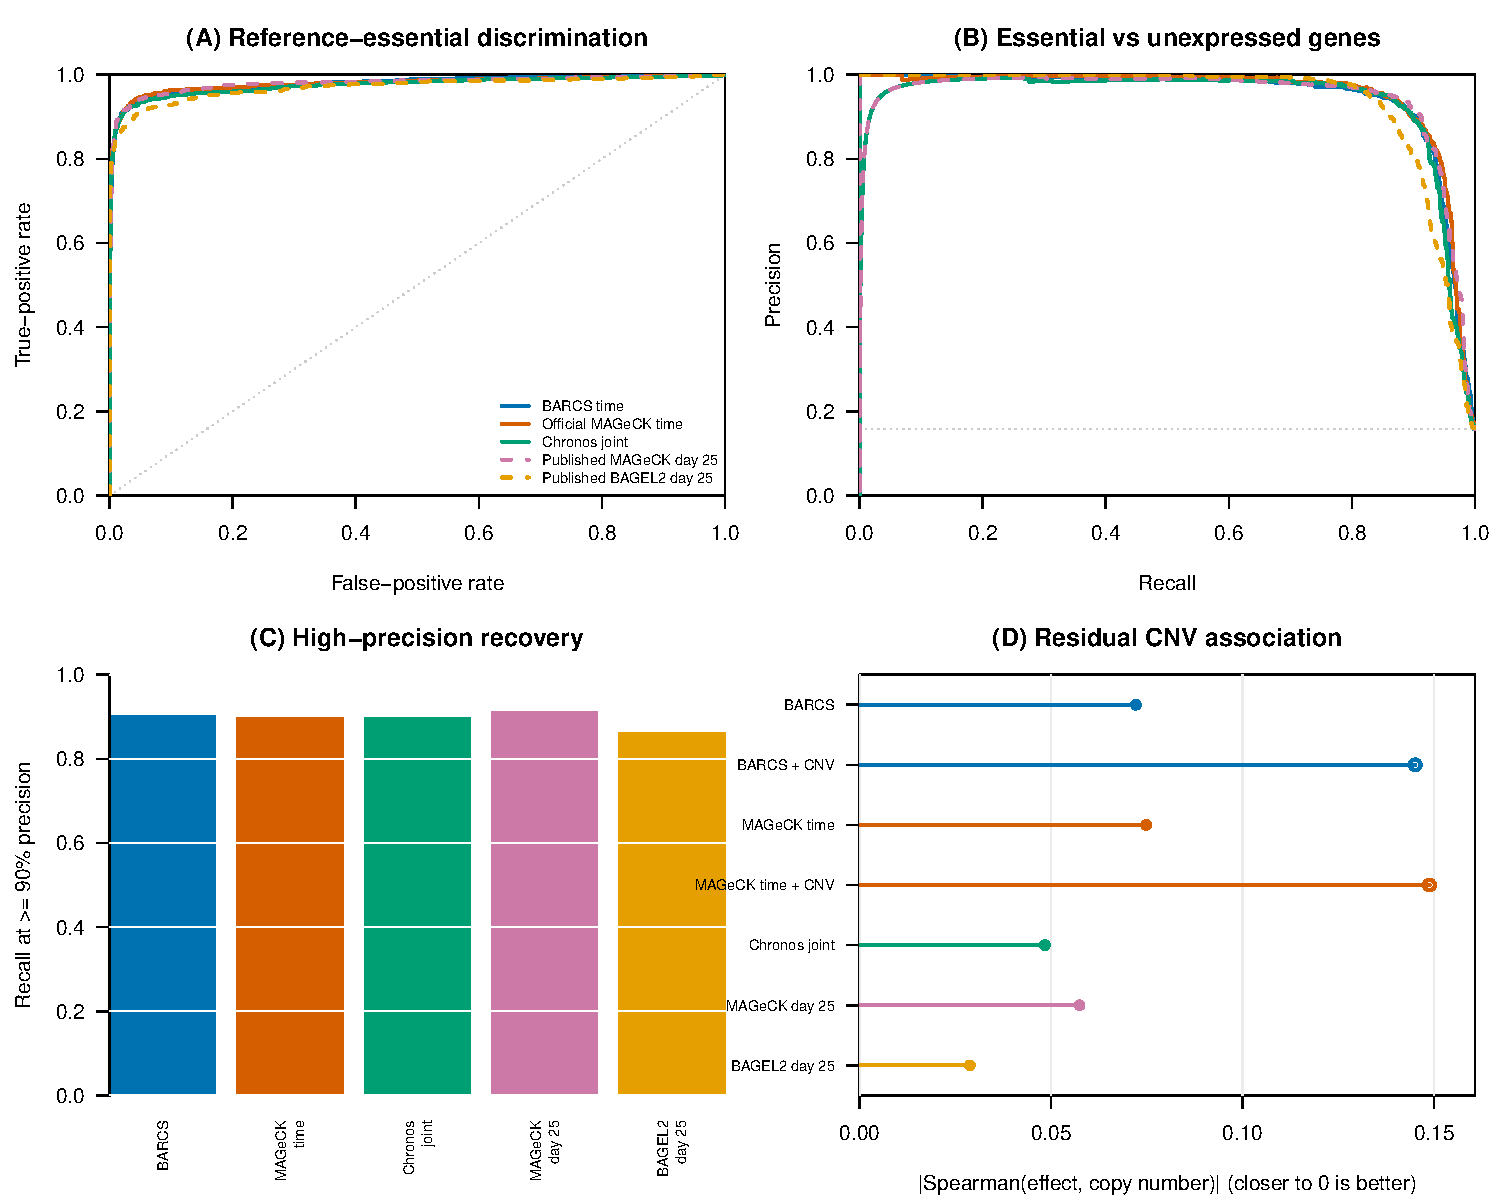
\includegraphics[width=\textwidth]{figures/chronos_tzelepis_benchmark.pdf}
\caption{Longitudinal HT-29 benchmark.  (A) ROC and (B) precision--recall
curves compare essential-gene recovery against unexpressed genes.  (C) Recall
at at least 90\% precision.  (D) Absolute residual effect--copy-number
association among unexpressed genes; values closer to zero are better.
Filled points are uncorrected results and open points are results after
official MAGeCK piecewise correction.  A method has the same color in every
panel.}
\label{fig:chronos}
\end{figure}
\clearpage

\subsubsection{What the longitudinal screen says about CNV correction}

We extracted the HT-29 profile (ACH-000552) from DepMap Public 20Q2
\citep{depmap20q2} and repeated the same copy-number audit used for A375.
Before correction, effect--copy-number Spearman correlation among unexpressed
genes is already small: $-0.072$ for BARCS, $-0.075$ for official
continuous-time MAGeCK, $-0.048$ for deposited Chronos joint effects,
$-0.046$ for the published MAGeCK average, and $-0.002$ for the published
BAGEL2 average.  The near-zero BAGEL2 association is a focused robustness
diagnostic, not evidence that BAGEL2 is the best classifier: Table
\ref{tab:chronos} shows that it has the lowest discrimination and
high-precision recovery on the same control-gene universe.
Applying MAGeCK 0.5.9.5's official piecewise normalizer makes the association
larger in absolute value rather than smaller: $-0.145$ for BARCS and $-0.149$ for
MAGeCK.  Thus the A375 result does not generalize automatically.

This failure mode is informative.  The piecewise correction estimates one
global effect--CNV trend across genes in one cell line and applies it after
model fitting.  When the nuisance association is weak and biological
dependencies are not exchangeable across copy-number regions, the fitted
trend can have the wrong practical target and over-correct null genes.
Chronos joint is shown without CNV correction because the published Chronos
procedure requires multiple cell lines to identify common essential genes and
was explicitly not applied to this single-line experiment
\citep{dempster2021chronos}.  The DepMap profile was measured separately from
the original screen, so cell-line drift is an additional limitation; the
result supports diagnosing correction rather than applying it by default.

\subsection{Processed-count boundary: Liang Cas13 fitness screens}

The five-cell-line Cas13 fitness study of \citet{liang2026lncrna} provides a
useful head-to-head boundary because it contains a specialist published
analysis, known-essential protein-coding controls, and cell-line-specific
non-expressed lncRNA null controls.  We used the deposited normalized Table S2
values requested for this comparison.  They are fractional after
median-of-ratios normalization, ComBat correction, and replicate-outlier
processing.  We rounded them once to the nearest pseudo-count and supplied
the identical matrix, with no additional normalization, to BARCS, official
MAGeCK-RRA, and official MAGeCK-MLE.  Liang RRA denotes the authors'
deposited \texttt{RobustRankAggreg} result and is not MAGeCK-RRA.

\begin{table}[ht]
\centering
\caption{Liang Cas13 processed-count sensitivity analysis, macro-averaged
over five cell lines.  Recall$_{5\%}$ fixes the empirical false-positive rate
among non-expressed lncRNA null controls at 5\%.  Calibration error is the
absolute difference between the observed null $p<0.05$ fraction and 0.05, so
lower is better.  The other four metrics are higher-is-better.  The best value
in each column is shown in bold and in its method color.}
\label{tab:liang}
\small
\setlength{\tabcolsep}{4pt}
\begin{tabular}{lrrrrr}
\toprule
Method & AUROC & Avg. precision & Recall$_{5\%}$ &
Calibration error & FDR$_{0.10}$ recall\\
\midrule
\methodswatch{mageckpink} Liang RRA &
  \textcolor{mageckpink}{\textbf{0.9703}} &
  \textcolor{mageckpink}{\textbf{0.8908}} &
  \textcolor{mageckpink}{\textbf{0.9167}} &
  \textcolor{mageckpink}{\textbf{0.0174}} &
  \textcolor{mageckpink}{\textbf{0.8233}}\\
\methodswatch{mageckorange} Official MAGeCK-RRA &
  0.9522 & 0.8425 & 0.8733 & 0.0181 & 0.7400\\
\methodswatch{mageckorange} Official MAGeCK-MLE &
  0.9508 & 0.8356 & 0.8600 & 0.0710 & 0.6800\\
\methodswatch{barcsblue} BARCS &
  0.9386 & 0.7756 & 0.8233 & 0.0274 & 0.4867\\
\bottomrule
\end{tabular}
\end{table}

Liang RRA leads every macro-averaged metric in
Table~\ref{tab:liang}; BARCS does not beat it.  At a common empirical 5\% null
false-positive rate, Liang RRA recovers 91.7\% of essential controls versus
82.3\% for BARCS.  At the 0.10 gene-FDR threshold, the gap widens
to 82.3\% versus 48.7\%.  The latter difference is consistent with
finite-sample conservatism: every cell line supplies only three or four
libraries, and the fitted day effect has one residual degree of freedom after
the intercept and available replicate block.  K562 is the sharpest example:
BARCS retains AUROC 0.911 but calls none of the essential controls at FDR
0.10.  More sequencing depth cannot replace the missing independent
libraries in a sample-level $t$ reference.

Official MAGeCK-RRA also modestly outperforms MAGeCK-MLE here.  Its null
calibration error is 0.018 compared with 0.071 for MLE, while its average
precision is 0.843 compared with 0.836.  This pattern supports a
design-specific interpretation: guide-rank aggregation is well matched to a
two-endpoint study with few replicates and already normalized inputs, whereas
a regression likelihood has little sample-level information from which to
estimate uncertainty.  It is not evidence that RRA is universally superior
to count regression.

Effect agreement remains substantial despite the threshold differences.
Within each cell line we computed Spearman correlation across all genes with
finite effects, then averaged the five correlations.  BARCS correlates 0.875
with MAGeCK-MLE, 0.864 with MAGeCK-RRA, and 0.784 with Liang RRA.  Thus the
principal BARCS deficit in this benchmark is not a reversal of the biological
ranking; it is reduced resolution and power under one residual degree of
freedom.

\begin{figure}[htbp]
\centering
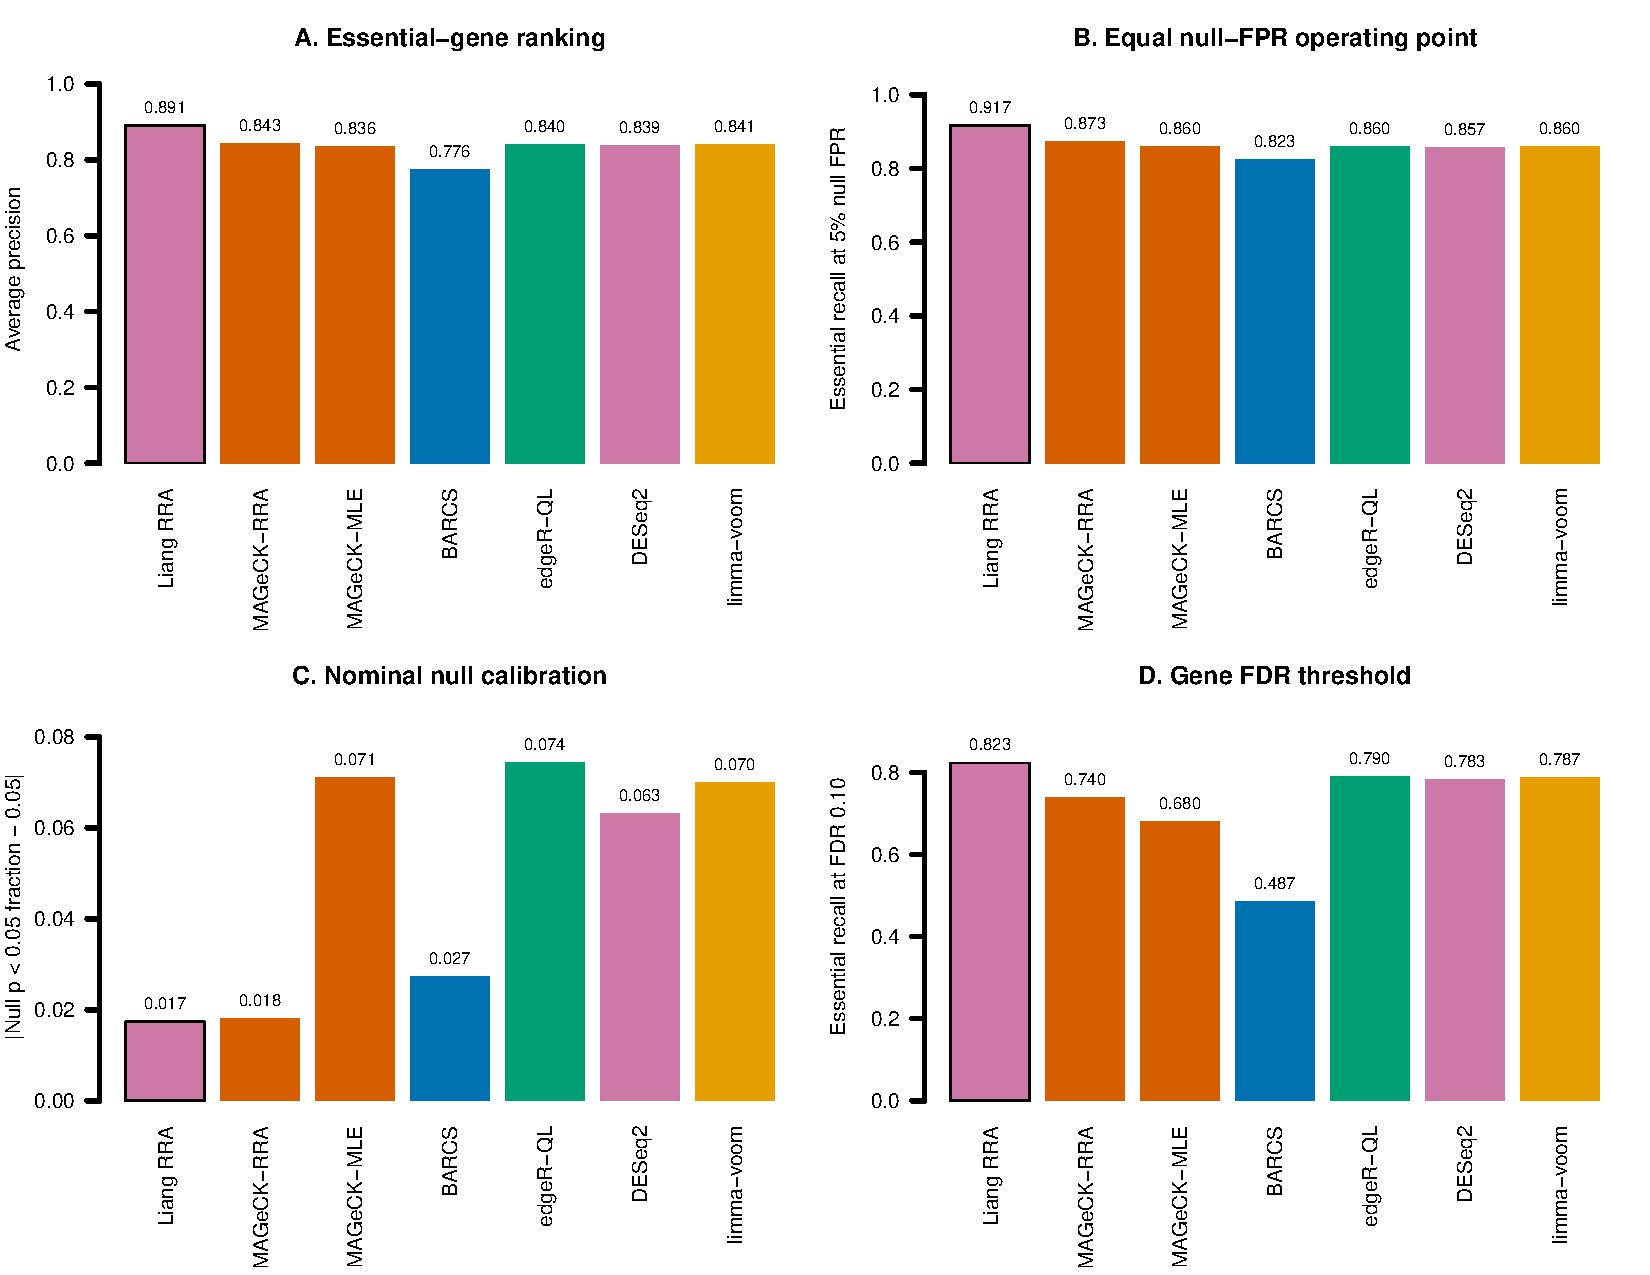
\includegraphics[width=\textwidth]{figures/liang_cas13_benchmark.pdf}
\caption{Liang Cas13 processed-count sensitivity analysis, macro-averaged
over five cell lines.  (A) Average precision for ranking essential controls
above non-expressed lncRNA nulls.  (B) Essential-control recall at a common
empirical 5\% null false-positive rate.  (C) Absolute error from the nominal
5\% null $p$-value rate; lower is better.  (D) Directional
essential-control recall at gene FDR 0.10.  A black
outline marks the best method in each panel.}
\label{fig:liang}
\end{figure}
\clearpage

This comparison has an important limit.  Rounding changes each deposited
value by only 0.25 on average and by less than 0.5 at most, but the values
were transformed before deposition.  Consequently, neither the
beta-binomial nor negative-binomial likelihood has its literal raw-count
sampling interpretation, and the nominal calibration panels are sensitivity
diagnostics rather than raw-count likelihood validation.  The reproducible
streaming pipeline supplied with BARCS makes a future raw-read confirmation
possible; until that is complete, the defensible conclusion is that the
published Liang RRA is the best fit to the deposited processed data.

\subsection{Stress test and model boundary: ordered-bin FACS}

The Waterbear study supplies a complementary continuous-phenotype benchmark
with unusually useful validation \citep{pimentel2024waterbear}.  GSE242880
contains a pooled CRISPR screen of IL2RA protein abundance in primary human
T cells.  Its low-coverage, high-MOI arm has four ordered FACS bins for each
of three donors, 6,000 guides targeting 1,350 genes or negative controls, and
26 regulators whose direction was confirmed by individual knockout and flow
cytometry.  Because these are primary donor cells rather than a cancer cell
line, this benchmark is not driven by tumor copy-number artifacts.

We assigned the four bins latent marker locations equal to the conditional
means of standard-normal intervals with the prespecified bin masses
$(0.2,0.3,0.3,0.2)$.  Beta-binomial regression used all 12 libraries with a
marker slope and donor indicators.  Official MAGeCK-MLE received the same
model space; its marker score was affinely mapped to zero--one because the
MAGeCK initializer requires a reference row with all non-intercept entries
zero.  We also fitted two outer-bin ablations and ran the paper's native
\texttt{mageck test} comparison of Q1 with Q4.

This design exposes a limitation of applying independent-library regression
to sorted data.  The four bins from one donor partition one cell pool and are
therefore negatively correlated, while the beta-binomial fit treats their
margins separately.  Among 593 non-targeting guides, the raw all-bin
beta-binomial $p<0.05$ frequency is 0.133.  We therefore added the
prespecified negative-control calibration implemented by
\texttt{bb\_calibrate\_controls()}: the empirical 95th percentile of absolute
control $t$ statistics is matched to the $t_8$ two-sided 0.05 cutoff, with
scales below one prohibited.  The estimated scale is 1.357; after calibration,
the non-targeting frequency is 0.049.  Estimates and the $t$ reference are
retained, while raw and calibrated inferential columns are both saved.

\begin{table}[ht]
\centering
\caption{GSE242880 low-coverage, high-MOI IL2RA FACS benchmark.  Recovery
uses each method's reported 0.10 discovery threshold and the independently
validated direction.  BARCS and MAGeCK use adjusted
$p$-values; Waterbear uses posterior inclusion probability above 0.90.
The non-targeting column is guide-level.  Waterbear and MAUDE values are
reported by the study and were not rerun.  The highest validated recovery and
the available non-targeting rate closest to 0.05 are highlighted.}
\label{tab:waterbear}
\small
\setlength{\tabcolsep}{4pt}
\begin{tabular}{lrrr}
\toprule
Method & Discoveries & Validated recovery & NTC $p<0.05$\\
\midrule
\methodswatch{barcsblue} BARCS, four bins + controls &
  49 & 22/26 & \textcolor{barcsblue}{\textbf{0.049}}\\
\methodswatch{barcsblue} BARCS, four bins raw & 127 & 23/26 & 0.133\\
\methodswatch{mageckorange} Official MAGeCK-MLE, four bins &
  72 & 17/26 & ---\\
\methodswatch{barcsblue} BARCS, outer bins & 34 & 18/26 & 0.064\\
\methodswatch{mageckorange} Official MAGeCK test, outer bins &
  32 & 18/26 & ---\\
\methodswatch{waterbearpurple} Waterbear, four bins (reported) &
  79 & 24/26 & ---\\
\methodswatch{maudered} MAUDE, four bins (reported) &
  406 & \textcolor{maudered}{\textbf{25/26}} & ---\\
\bottomrule
\end{tabular}
\end{table}

The calibrated four-bin BARCS result recovers four more
validated regulators than all-bin MAGeCK-MLE while making 23 fewer calls.  It
is two regulators behind the reported Waterbear result and three behind MAUDE.
The raw 23/26 BARCS result is not the primary claim because
its negative controls reveal inflation.  MAUDE's 25/26 recovery is also not
evidence of superior specificity: it calls 406 of 1,350 genes, and the
Waterbear study found poor MAUDE calibration in simulations
\citep{pimentel2024waterbear,deboer2020maude}.  Across all 1,350 genes,
uncalibrated BARCS and MAGeCK-MLE all-bin effects have
Spearman correlation 0.917, so the recovery difference is not caused by
globally incompatible directions.  All 26 validation effects have the
expected sign under each independently rerun method.

The follow-up table contains more information than the 26-positive subset.
Thirty-three candidates were tested individually: 26 had a concordant IL2RA
effect and seven did not validate.  Restricting evaluation to these measured
labels avoids the incorrect assumption that every other screen gene is a false
positive.  Table~\ref{tab:waterbearpanel} reports threshold and ranking metrics
for the five methods rerun here.

\begin{table}[ht]
\centering
\caption{Classification in the selected 33-gene experimental follow-up panel
(26 concordant positives and seven non-validating candidates).  This panel is
small and was selected from a previous screen, so the metrics are supporting
evidence rather than unbiased genome-wide performance estimates.  Higher is
better for every metric; column maxima are highlighted.}
\label{tab:waterbearpanel}
\small
\setlength{\tabcolsep}{4pt}
\begin{tabular}{lrrrrr}
\toprule
Method & F1 & MCC & Balanced accuracy & AUROC & Avg. precision\\
\midrule
\methodswatch{barcsblue} BARCS, four bins + controls
  & \textcolor{barcsblue}{\textbf{0.863}}
  & \textcolor{barcsblue}{\textbf{0.398}}
  & \textcolor{barcsblue}{\textbf{0.709}} & 0.808 & 0.945\\
\methodswatch{barcsblue} BARCS, four bins raw
  & 0.852 & 0.194 & 0.585
  & \textcolor{barcsblue}{\textbf{0.819}}
  & \textcolor{barcsblue}{\textbf{0.950}}\\
\methodswatch{mageckorange} Official MAGeCK-MLE, four bins
  & 0.723 & 0.070 & 0.541 & 0.626 & 0.872\\
\methodswatch{barcsblue} BARCS, outer bins
  & 0.783 & 0.340 & 0.703 & 0.714 & 0.913\\
\methodswatch{mageckorange} Official MAGeCK test, outer bins
  & 0.766 & 0.224 & 0.632 & 0.703 & 0.906\\
\bottomrule
\end{tabular}
\end{table}

The raw four-bin model has the strongest rank metrics, which indicates that the
continuous trend is extracting useful signal.  Control calibration changes the
decision boundary rather than the estimated effects and produces the best F1,
Matthews correlation, and balanced accuracy in the validation panel.  That
combination is the central evidence for BARCS here:
continuous-bin ranking gains are retained while explicit null guides prevent
the extra calls from being mistaken for confidence.

This benchmark is stronger than a rank-correlation-only comparison because it
contains directionally validated biology and hundreds of explicit null
guides.  It is not an unbiased precision experiment: the 26 genes were chosen
for follow-up from an earlier screen, and unvalidated genes cannot simply be
called false positives.  Nor does it overturn Waterbear's modeling advantage.
Waterbear represents the joint multinomial bin structure, uncertain cutoffs,
guide-to-gene hierarchy, and sparse effects; BARCS supplies
a much faster transparent trend test but needs negative controls here to
diagnose and scale inference under a violated independence assumption.  The deposited paper reports
24/26 for Waterbear and 17/26 for MAGeCK; the independent current
\texttt{mageck test} rerun gives 18/26, a one-gene implementation-level
difference.

These results separate three meanings of ``better.''  First, ranking quality
asks whether validated regulators move toward the top; the raw four-bin model
performs strongly by AUROC and average precision.  Second, decision quality
asks whether a prespecified threshold balances recovery and false calls; the
control-calibrated model leads the rerun methods by F1 and Matthews
correlation.  Third, likelihood fidelity asks whether the sampling dependence
is represented; Waterbear wins that design question because it models all bins
from a donor jointly.  BARCS is compelling here because it
does well on the first two questions with a simple general-purpose model and
also provides the control diagnostic that exposes the third.

The published Waterbear and MAUDE aggregates cannot be assigned validation-
panel F1 or Matthews correlation without their gene-level calls for all seven
non-validating candidates.  Reporting 24/26 or 25/26 as if it were complete
accuracy would therefore mix sensitivity with an unknown precision.  We retain
those values as positive-control recovery references and restrict
classification metrics to the methods rerun from complete outputs.

\begin{figure}[ht]
\centering
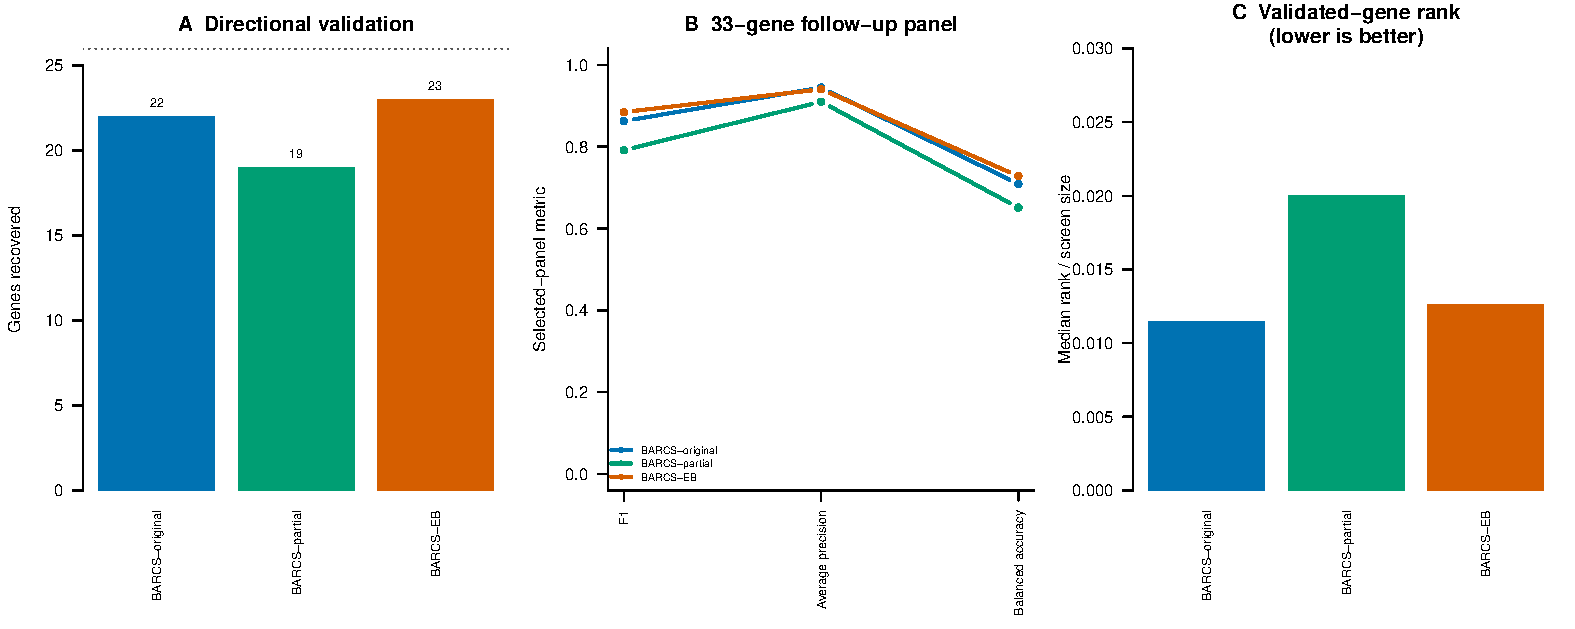
\includegraphics[width=\textwidth]{figures/waterbear_facs_benchmark.pdf}
\caption{Ordered-bin IL2RA FACS benchmark.  (A) Positive-control recovery for
all methods.  (B) F1 in the selected 33-gene panel for methods rerun here.
(C) All-bin BARCS and MAGeCK-MLE effects, with validated genes highlighted.
(D) Non-targeting-guide empirical null curves, showing the correction of raw
all-bin inflation.}
\label{fig:waterbear}
\end{figure}
\clearpage

\subsection{Genome-scale FACS simulation: does dispersion moderation change
the calibration--power tradeoff?}

To isolate the FACS design and estimation questions from the
candidate-selected Waterbear validation set, we used CRISPulator 0.5.1
\citep{nagy2017crispulator} to simulate CRISPR knockout screens with known
gene effects at genome scale.  Each of three prespecified seeds generated
10,000 genes, five guides per gene, and four independent screen replicates,
for 50,000 guides per screen.  Twenty percent of genes changed the latent
phenotype and 5\% were explicit negative controls.  The stress-test setting
used phenotype noise $\sigma=2$, 50 sorted cells per guide, and 50 reads per
guide per sample.  Multiplicity of infection was 0.20 in the main analysis
and 0.30 in the supplementary analysis: 0.20 is the operating point at which
the single-integration approximation shared by all of these guide-level
models is most defensible, and 0.30 stresses it.

Each replicate produced a low 0--25\% tail, a high 75--100\% tail, and an
unsorted 0--100\% bulk sample.  The two tails were assigned the conditional
standard-normal locations $-1.271$ and $1.271$; bulk was assigned zero.
Replicate indicators were included in every fit.  We compared this
three-sample fit with the two-tail ablation.  Importantly, ``three sample''
does not mean three independent bins: the bulk sample contains the cell
populations from both tails and costs 50\% more sequencing than the tail-only
design.

Two BARCS gene statistics are carried here.  BARCS-ST
(\texttt{BARCS-original}) is the historical calibrated signed-$z$ statistic.
BARCS-MOD (\texttt{BARCS-moderated}) reuses the same guide fits after
guide-dispersion moderation, which shrinks each guide's variance inflation
toward a library-wide trend before the same signed-$z$ aggregation.  At
genome scale the moderation prior is estimated from 50,000 guides and is
correspondingly sharp: the fitted prior degrees of freedom were 42.7--45.8
against the seven residual degrees of freedom the design itself supplies.

\begin{table}[ht]
\centering
\caption{Genome-scale CRISPulator FACS benchmark at MOI 0.20, 10,000 genes
and 50,000 guides, over three fixed simulation seeds (mean $\pm$ standard
deviation).  Recall counts active genes called at gene FDR 0.10 with the
correct direction.  FDP is the realized fraction of inactive genes among
calls; the nominal target is 0.10.  Column maxima for ranking, effect
recovery, recall, and F1 are highlighted, as is the FDP closest to nominal
from below.  MAGeCK-MLE could not be refitted at these settings in the
analysis environment and is reported at 400 genes elsewhere.}
\label{tab:crispulator}
\small
\setlength{\tabcolsep}{3pt}
\resizebox{\textwidth}{!}{%
\begin{tabular}{llrrrrrr}
\toprule
Method & Samples & AUROC & Avg.\ precision & Effect $\rho_s$ &
Directional recall & FDP & F1\\
\midrule
\methodswatch{barcsblue} BARCS-ST & Low--bulk--high &
0.947$\pm$.004 & 0.899$\pm$.007 & 0.924$\pm$.004 &
0.716$\pm$.022 & 0.068$\pm$.006 & 0.810$\pm$.012\\
\methodswatch{mageckorange} BARCS-MOD & Low--bulk--high &
\textcolor{mageckorange}{\textbf{0.954$\pm$.003}} &
\textcolor{mageckorange}{\textbf{0.916$\pm$.005}} &
\textcolor{mageckorange}{\textbf{0.924$\pm$.004}} &
0.774$\pm$.014 & 0.071$\pm$.002 &
\textcolor{mageckorange}{\textbf{0.845$\pm$.008}}\\
\methodswatch{chronosgreen} edgeR-QL + Stouffer & Low--bulk--high &
0.953$\pm$.003 & 0.913$\pm$.005 & 0.923$\pm$.003 &
0.857$\pm$.012 & 0.216$\pm$.002 & 0.819$\pm$.005\\
\methodswatch{mageckpink} DESeq2 + Stouffer & Low--bulk--high &
0.953$\pm$.003 & 0.914$\pm$.005 & 0.923$\pm$.003 &
\textcolor{mageckpink}{\textbf{0.869$\pm$.012}} &
0.252$\pm$.002 & 0.804$\pm$.004\\
\methodswatch{bagelgold} limma-voom + Stouffer & Low--bulk--high &
0.954$\pm$.003 & 0.914$\pm$.004 & 0.924$\pm$.003 &
0.862$\pm$.011 & 0.227$\pm$.002 & 0.815$\pm$.004\\
\midrule
\methodswatch{barcsblue} BARCS-ST & Low--high &
0.941$\pm$.004 & 0.883$\pm$.009 & 0.923$\pm$.004 &
0.615$\pm$.013 & 0.043$\pm$.001 & 0.749$\pm$.010\\
\methodswatch{mageckorange} BARCS-MOD & Low--high &
0.955$\pm$.003 & 0.917$\pm$.005 & 0.923$\pm$.004 &
0.776$\pm$.012 & 0.068$\pm$.004 & 0.847$\pm$.007\\
\bottomrule
\end{tabular}
}
\end{table}

At genome scale the tradeoff resolves rather than persisting.  Guide-dispersion
moderation makes BARCS-MOD the best method on every truth-recovery metric in
the low--bulk--high design while leaving its realized FDP below the nominal
target.  Paired over the three seeds, BARCS-MOD exceeds edgeR-QL in average
precision by 0.0027 (95\% interval 0.0020 to 0.0034) and in F1 by 0.026 (0.014
to 0.038); the corresponding F1 margins are 0.040 over DESeq2 and 0.030 over
limma-voom, and every one of these intervals excludes zero.  The three general
count models still recover more active genes in raw directional recall,
0.857--0.869 against 0.774, but they do so at realized FDP 0.216--0.252, more
than twice the nominal 0.10 target after the common Stouffer gene summary.
Their extra recall is therefore not a calibrated win, and it costs them F1.
BARCS-MOD holds FDP at 0.071 and a negative-control gene $p<0.05$ frequency of
0.053, against 0.125--0.135 for the count models.

The gain over the historical statistic is also unambiguous, and it is a gain
in ranking rather than a threshold effect: average precision rises from 0.899
to 0.916, a paired difference of 0.017 (0.011 to 0.023), and F1 from 0.810 to
0.845, with realized FDP statistically unchanged.  This is the expected
consequence of estimating the moderation prior from 50,000 guides: a guide
whose own seven residual degrees of freedom understate its variance is
corrected individually, so the negative-control calibration no longer has to
answer those guides with one penalty applied to the whole screen.

Bulk does not supply a new directional contrast.  Across seeds, the
low--bulk--high and tail-only gene effects have mean Spearman correlation
above 0.998.  For the historical statistic its practical contribution is to
the fitted baseline, dispersion, and residual degrees of freedom: mean
directional recall rises from 0.615 to 0.716 and F1 from 0.749 to 0.810, at
50\% more reads.  Moderation largely removes that dependence.  BARCS-MOD
reaches F1 0.847 on the two tails alone against 0.845 with bulk added, so the
information the bulk sample was supplying to the variance model is recovered
more cheaply by borrowing it across the library.  Because the bulk pool
overlaps the tails, its apparent inferential gain may in any case partly
reflect an independence approximation rather than new biological information;
that reading is strengthened by its being replaceable.

At MOI 0.30 every one of these conclusions is reproduced
(Supplementary Table~\ref{tab:crispulator-moi03}): BARCS-MOD again leads
average precision and F1 with all paired intervals excluding zero, at FDP
0.074 against 0.212--0.249 for the count models.

\begin{table}[ht]
\centering
\caption{Supplementary: the same genome-scale CRISPulator FACS benchmark at
MOI 0.30 rather than 0.20, over the same three seeds (mean $\pm$ standard
deviation).  A higher multiplicity of infection stresses the
single-integration approximation shared by every guide-level model compared
here.  Column highlighting follows Table~\ref{tab:crispulator}.}
\label{tab:crispulator-moi03}
\small
\setlength{\tabcolsep}{3pt}
\resizebox{\textwidth}{!}{%
\begin{tabular}{llrrrrrr}
\toprule
Method & Samples & AUROC & Avg.\ precision & Effect $\rho_s$ &
Directional recall & FDP & F1\\
\midrule
\methodswatch{barcsblue} BARCS-ST & Low--bulk--high &
0.947$\pm$.001 & 0.900$\pm$.003 & 0.923$\pm$.003 &
0.742$\pm$.007 & 0.078$\pm$.009 & 0.822$\pm$.001\\
\methodswatch{mageckorange} BARCS-MOD & Low--bulk--high &
\textcolor{mageckorange}{\textbf{0.955$\pm$.002}} &
\textcolor{mageckorange}{\textbf{0.917$\pm$.003}} &
\textcolor{mageckorange}{\textbf{0.923$\pm$.003}} &
0.784$\pm$.008 & 0.074$\pm$.004 &
\textcolor{mageckorange}{\textbf{0.849$\pm$.003}}\\
\methodswatch{chronosgreen} edgeR-QL + Stouffer & Low--bulk--high &
0.954$\pm$.002 & 0.915$\pm$.002 & 0.922$\pm$.003 &
0.855$\pm$.002 & 0.212$\pm$.006 & 0.820$\pm$.003\\
\methodswatch{mageckpink} DESeq2 + Stouffer & Low--bulk--high &
0.954$\pm$.002 & 0.916$\pm$.003 & 0.921$\pm$.003 &
\textcolor{mageckpink}{\textbf{0.871$\pm$.003}} &
0.249$\pm$.011 & 0.807$\pm$.005\\
\methodswatch{bagelgold} limma-voom + Stouffer & Low--bulk--high &
0.954$\pm$.002 & 0.915$\pm$.003 & 0.923$\pm$.003 &
0.858$\pm$.007 & 0.224$\pm$.001 & 0.815$\pm$.004\\
\midrule
\methodswatch{barcsblue} BARCS-ST & Low--high &
0.941$\pm$.001 & 0.884$\pm$.002 & 0.923$\pm$.003 &
0.616$\pm$.012 & 0.036$\pm$.004 & 0.752$\pm$.008\\
\methodswatch{mageckorange} BARCS-MOD & Low--high &
0.956$\pm$.002 & 0.919$\pm$.003 & 0.923$\pm$.003 &
0.778$\pm$.003 & 0.063$\pm$.002 & 0.850$\pm$.001\\
\bottomrule
\end{tabular}
}
\end{table}

\paragraph{Supporting 400-gene sensitivity to MOI, guide quality, library
size, and replication.}
The remaining simulation analyses in this subsection are the earlier
400-gene grid, retained because they map the parameter boundaries that the
genome-scale benchmark deliberately does not vary, including the
one-replicate boundary.  They predate the moderated statistic and use the
historical BARCS-ST default and the earlier
$\mathrm{MOI}\in\{0.10,0.25,0.40\}$ levels, so they should be read as
boundary mapping rather than as the headline comparison.  We
varied MOI, the high-quality-guide fraction, the number of genes, and the
number of independent screen replicates one at a time, using five paired seeds
at every setting (ten unique settings and 50 simulations in total).  Nine
settings had at least three replicates; the one-replicate setting was a
prespecified diagnostic boundary.  Among the supported settings, in the
primary low--bulk--high comparison,
BARCS-minus-MAGeCK-MLE average precision ranged only from $-0.015$ to $0.022$
and changed sign across settings.  Thus this experiment does not support a
general ranking advantage for BARCS.  Its more consistent strength was
directional recovery at the prespecified FDR threshold: the directional-recall
difference was positive in seven of nine settings and ranged from $-0.018$ to
$0.136$, while the F1 difference ranged from $-0.022$ to $0.080$.

The largest directional-recall differences occurred at MOI 0.10
($+0.107$) and a high-quality-guide fraction of 0.75 ($+0.119$).  At MOI
0.40, however, MAGeCK-MLE led directional recall by $0.018$ and F1 by
$0.022$; with only 60\% high-quality guides, the methods were nearly tied on
directional recall and MAGeCK-MLE led F1 by $0.005$.  Across 100, 400, and
1,000 genes, BARCS directional-recall differences were $+0.081$, $+0.047$,
and $+0.064$, respectively, whereas average-precision differences again
remained small.  The 100-gene setting also produced realized FDP above 0.10
for both methods (0.181 for BARCS and 0.147 for MAGeCK-MLE), warning that five
small-library replicates do not establish finite-sample FDR control.  These
results sharpen the claim: BARCS can improve directionally correct thresholded
recovery under some noisy or low-MOI conditions, but neither method dominates
every metric or simulation regime.

Replication changed that comparison.  With three replicates, BARCS exceeded
MAGeCK-MLE in directional recall by 0.136 and F1 by 0.080; with four
replicates the differences were 0.047 and 0.011.  At six replicates the signs
reversed slightly, to $-0.012$ for directional recall and $-0.014$ for F1.
The practical interpretation is not that fewer replicates are desirable:
average precision, recall, and F1 increased for both methods as replication
increased.  Rather, BARCS's relative sensitivity is largest in the
low-replication regime, whereas MAGeCK-MLE catches up when information is
abundant.

One replicate crossed from low information into non-confirmatory inference.
Ordinary BARCS retained higher average precision than MAGeCK-MLE, 0.633 versus
0.548, but made no discoveries at gene FDR 0.10 across the five seeds;
MAGeCK-MLE's mean directional recall was only 0.014.  The new BARCS-GC
guide-consistency statistic increased average precision to 0.670,
directional recall to 0.145, and F1 to 0.245.  It made 58 calls across the
five simulations (3--19 per seed), all of which were active genes under the
simulated truth, for mean realized FDP 0.  The fitted empirical-null scales
were 2.19--2.60, showing why an unscaled Wald reference would have been
anti-conservative.

This improvement is useful but deliberately narrow.  BARCS-GC asks whether
independently designed guides give concordant signed effects and assumes that
fewer than half of genes are active; it does not create biological replication.
Its empirical-null calls are therefore hypothesis-generating, not
confirmatory.  edgeR-QL and limma-voom reported mean directional recall of
0.708 and 0.684 in the same data, but their mean realized FDP was 0.526 and
0.507.  DESeq2 was less inflated (FDP 0.141), yet still exceeded the nominal
0.10 target.  We recommend an independent screen for confirmation even when
BARCS-GC is used to prioritize genes from an otherwise irreplaceable $R=1$
experiment.


\begin{figure}[!t]
\centering
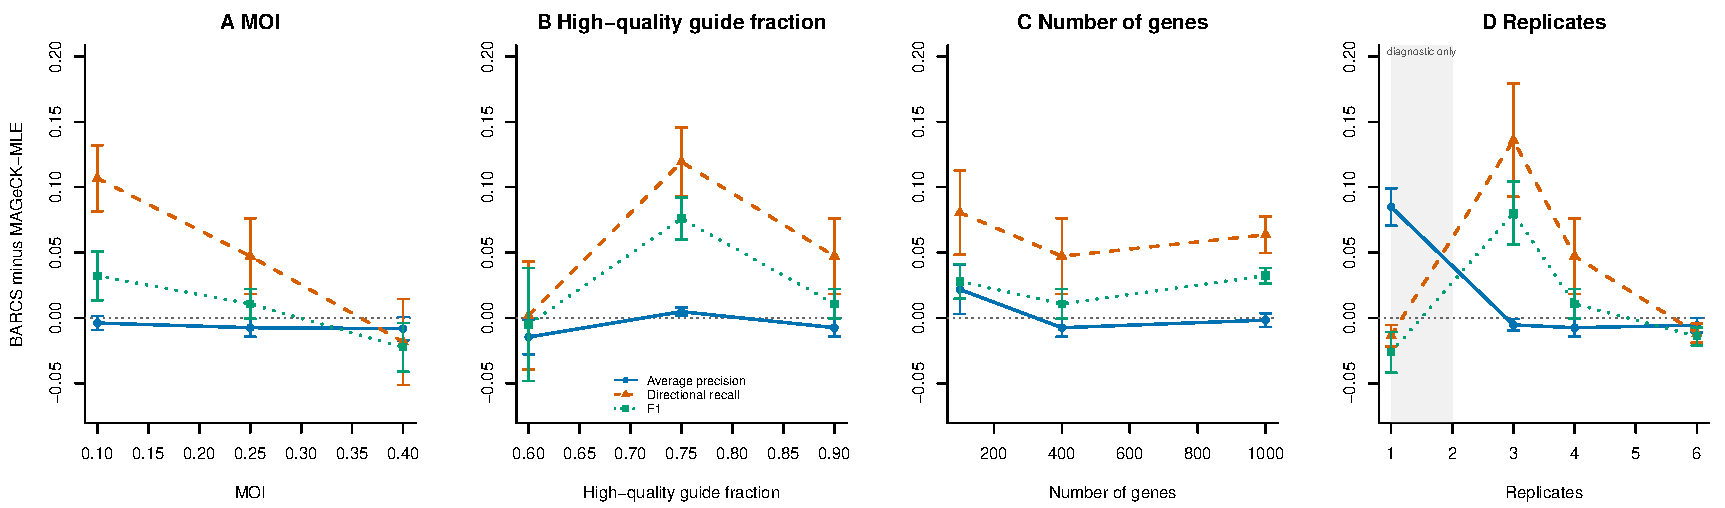
\includegraphics[width=\textwidth]{figures/crispulator_facs_parameter_sensitivity.pdf}
\caption{Paired parameter sensitivity across five seeds per setting.
Points show mean BARCS-minus-MAGeCK-MLE differences in the low--bulk--high
design, with standard-error bars.  Positive values favor BARCS.  Each panel
varies (A) MOI, (B) high-quality-guide fraction, (C) number of genes, or
(D) independent screen replicates while holding the other parameters at their
baseline values.  Ranking differences remain close to zero, whereas
directional-recall differences are usually positive but reverse at MOI 0.40
and six replicates.  The shaded $R=1$ region is a diagnostic boundary and not
a recommended confirmatory design.}
\label{fig:crispulator-sensitivity}
\end{figure}

\paragraph{Multiple count models expose the calibration--power tradeoff.}
Across the nine supported scenarios with $R\geq3$, mean realized FDP was 0.094
for BARCS and 0.064 for
MAGeCK-MLE, compared with 0.250 for edgeR-QL plus Stouffer, 0.243 for DESeq2
plus Stouffer, and 0.230 for limma-voom plus Stouffer.  Figure~
\ref{fig:crispulator-external} makes the consequence visible.  The general
count models attain excellent average precision and raw directional recall,
but their apparent recall advantage is coupled to FDP near 0.20--0.25.
Restricted to these supported settings, their F1 advantage over BARCS is not
resolvable: the paired differences are $+0.008$ for edgeR-QL (95\% interval
$-0.015$ to $+0.030$), $+0.013$ for DESeq2 ($-0.010$ to $+0.035$), and
$+0.014$ for limma-voom ($-0.008$ to $+0.037$), whereas the paired
average-precision advantage of $0.016$--$0.017$ remains clear.  At six
replicates, BARCS and MAGeCK-MLE reach F1 of 0.893 and 0.907 while keeping mean
FDP at 0.079 and 0.064; edgeR-QL, DESeq2, and limma-voom reach F1 of
0.840--0.862 with FDP of 0.196--0.235.  This is evidence for the value of a
CRISPR-aware gene-testing and calibration pipeline, not evidence that the
general count models rank genes poorly.

\begin{figure}[!t]
\centering
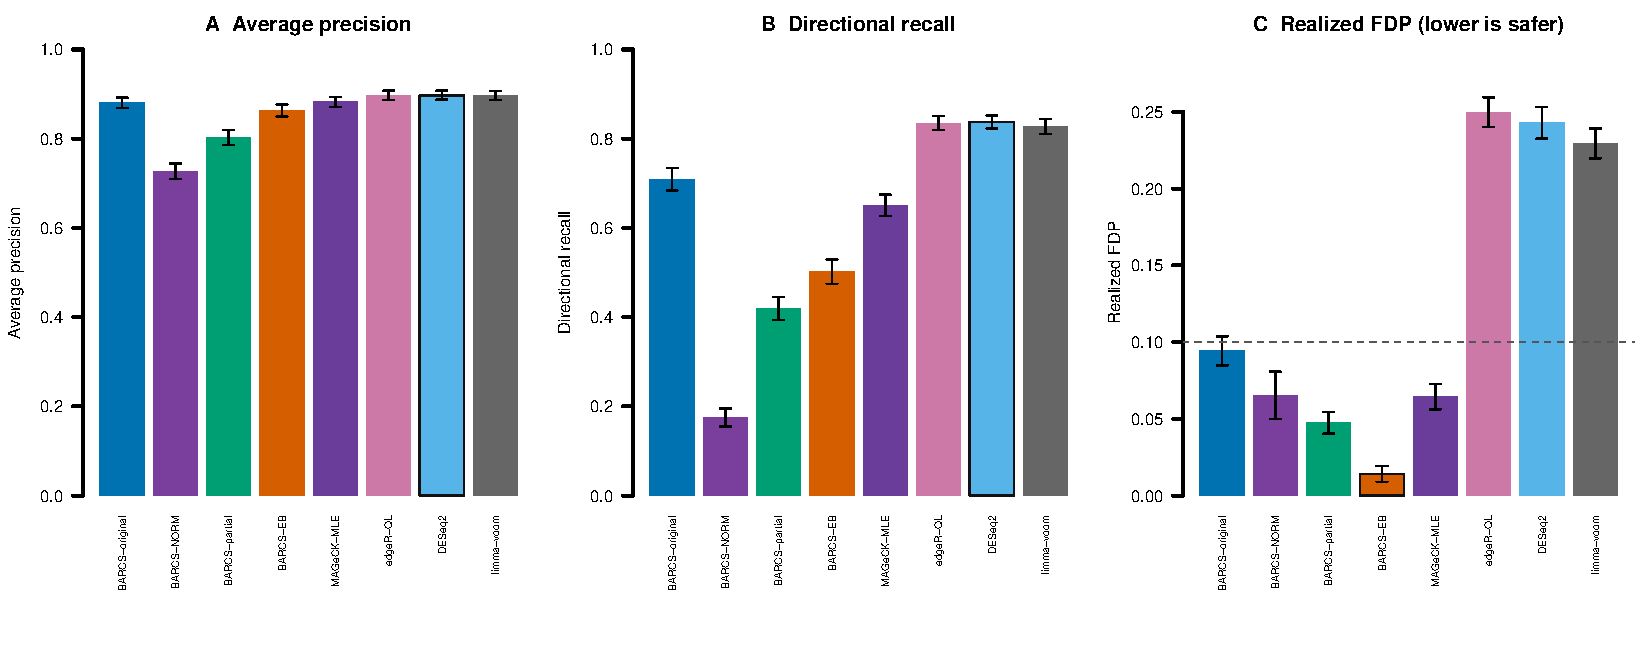
\includegraphics[width=\textwidth]{figures/crispulator_facs_external_head_to_head.pdf}
\caption{Head-to-head comparison across the 45 multi-replicate low--bulk--high
CRISPulator runs.  The one-replicate setting is a prespecified diagnostic
boundary and is excluded here; it is reported separately in the text.
Bars are means and error bars are standard errors.  (A) Average
precision, (B) directionally correct recall at gene FDR 0.10, and (C) realized
FDP, where lower is safer and the dotted line is the nominal 0.10 target.
edgeR-QL, DESeq2, and limma-voom use the common directional Stouffer gene
summary; MAGeCK-MLE uses its native gene model.}
\label{fig:crispulator-external}
\end{figure}

\noindent\begin{minipage}{\textwidth}
At the four-replicate baseline, mean core fitting times were 0.35 seconds for
BARCS, 4.34 seconds for MAGeCK-MLE, 0.24 seconds for edgeR-QL, 0.92 seconds for
DESeq2, and 0.06 seconds for \mbox{limma-voom}.  These measurements exclude
simulation, file input/output, and guide-to-gene aggregation; they show that
the broader comparison is computationally practical but should not be read as
an end-to-end software benchmark.
\end{minipage}

\clearpage
\subsection{Backward compatibility: GSE70038}

GSE70038 contains 64,747 guides measured in 16 libraries from two glioblastoma
stem-cell lines and two neural stem-cell lines, with duplicate initial and
terminal samples \citep{toledo2015pkmyt1}.  This binary terminal-versus-initial
setting is a special case of the regression model, not a continuous-phenotype
benchmark.  It is nevertheless useful because it provides published biology
and permits an exact design-matched comparison with MAGeCK-MLE.

We followed the design-matrix rules in Table~5 and Box~3 of the MAGeCKFlute
protocol \citep{wang2019mageckflute}.  The first column is one for every
library; each initial library has zeros elsewhere; and each terminal library
has one in exactly one of four cell-line columns.  The same $16\times5$ matrix
was supplied to beta-binomial regression and the official MAGeCK-MLE 0.5.9.5
executable.  MAGeCK used median normalization and its Wald inference.  For the
beta-binomial result, guide effects were summarized by their within-gene
median, and directional guide $p$-values were combined by Stouffer's method.
This aggregation is an explicit comparison device, not a proposed replacement
for MAGeCK's gene model.

The ``effect rank correlation'' reported below is calculated in this analysis,
not copied from GEO or the MAGeCKFlute paper.  Separately for each terminal
coefficient, we pair all genes available from both methods.  The
beta-binomial effect is the within-gene median guide coefficient, and the
MAGeCK effect is its official MLE beta.  We assign average ranks to these two
effect vectors and take their Pearson correlation, which is exactly Spearman's
rank correlation.  The 18,077 paired effects and their ranks for every
coefficient are written to
\texttt{results/gse70038/effect\_concordance\_pairs.csv.gz}.

\begin{table}[ht]
\centering
\caption{Effect concordance between \methodswatch{barcsblue} BARCS and
\methodswatch{mageckorange} official MAGeCK-MLE on GSE70038.  Jaccard is the
overlap divided by the union of the 200 most depleted genes from each method.
Higher agreement is better; column maxima are shown in bold.}
\label{tab:gse}
\begin{tabular}{lrr}
\toprule
Terminal coefficient & Spearman effect correlation & Top-200 Jaccard\\
\midrule
GSC0131 & \textbf{0.928} & 0.550\\
GSC0827 & 0.888 & 0.533\\
NSCCB660 & 0.905 & 0.544\\
NSCU5 & 0.915 & \textbf{0.562}\\
\bottomrule
\end{tabular}
\end{table}

The comparison is not circular: beta-binomial regression conditions on each
library total, whereas MAGeCK uses a normalized negative-binomial count model
with guide-efficiency estimation \citep{li2015mageckvispr}.  Despite those
differences, all four effect correlations exceed 0.88.  These correlations
measure agreement of the inferred gene ordering; they are not likelihood,
calibration, or predictive-fit statistics and therefore cannot identify a
better-fitting method.  In GSC0131, the
published convergent dependency PKMYT1 has effect $-0.987$ and FDR
$1.87\times10^{-8}$ under beta-binomial regression, versus beta $-0.786$ and
Wald FDR $4.53\times10^{-8}$ under MAGeCK-MLE.  Both also recover HEATR1,
TFAP2C, and WEE1 depletion.  Figure~\ref{fig:gse} shows the complete GSC0131
comparison; the reproducible PDF contains one page per terminal coefficient.

\begin{figure}[ht]
\centering
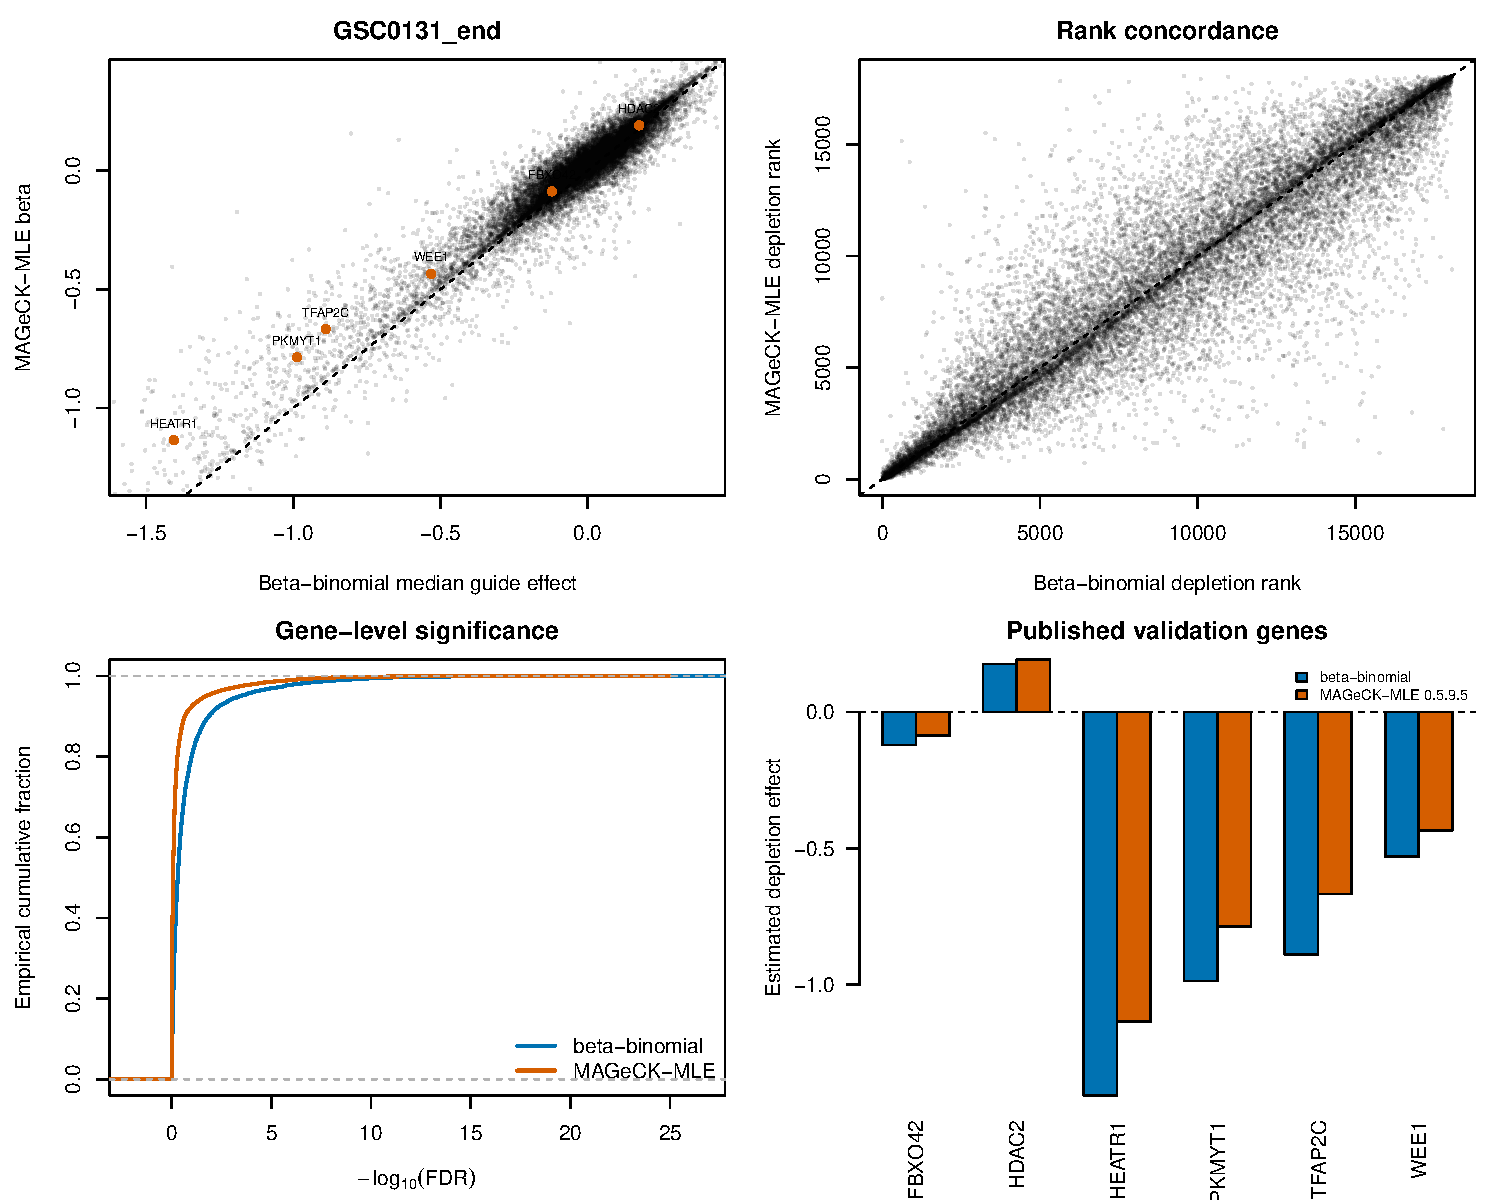
\includegraphics[width=\textwidth]{figures/gse70038_head_to_head.pdf}
\caption{GSE70038 GSC0131 head-to-head.  (A) Gene effects, with dark points
marking the prespecified genes PKMYT1, HEATR1, TFAP2C, FBXO42, HDAC2, and WEE1.
(B) Depletion-rank concordance.  (C) Gene-level FDR distributions.  (D)
Effects for the published validation genes.}
\label{fig:gse}
\end{figure}
\clearpage

\subsection{Endpoint benchmark and copy-number audit}

To ask which method ranks biological dependencies better, we used the
Brunello A375 negative-selection screen of \citet{sanson2018optimized}, bundled
with CB\textsuperscript{2}.  This is an ordinary endpoint screen rather than a
continuous-phenotype experiment, but it supplies an external target unavailable
in GSE70038: reference essential genes should rank ahead of reference
nonessential genes.  The beta-binomial score combines guide
evidence by directional Stouffer aggregation; the MAGeCK score uses the
official MLE beta and Wald $p$-value.  Both are oriented so larger scores mean
stronger depletion.

\subsubsection{Copy-number-aware analysis}

Copy number is a gene-level property of A375, not a sample-level covariate:
for a given guide it is constant across the plasmid and three terminal
libraries.  Adding it directly to the four-row sample design would therefore
be non-identifiable with the endpoint effect.  Instead, we downloaded the
A375 gene-level profile (ACH-000219) from DepMap Public 19Q3
\citep{depmap19q3,meyers2017cnv} and used MAGeCK 0.5.9.5's official
\texttt{--cnv-norm} piecewise correction.  For an apples-to-apples comparison,
the same MAGeCK piecewise normalizer was applied to the beta-binomial
within-gene median effects.  It adjusts effect sizes after model fitting; it
does not refit either count likelihood.  The common CNV-complete evaluation set
contains 1,506 essential and 869 nonessential genes.

\begin{table}[ht]
\centering
\caption{CNV-aware Sanson A375 benchmark.  The final column is Spearman
correlation between effect and copy number among reference nonessential genes;
values nearer zero indicate less residual CNV-associated depletion.  F1 uses
nominal FDR 0.05 and a negative effect.  Higher discrimination metrics and
CNV correlation closest to zero are highlighted.}
\label{tab:sanson}
\small
\setlength{\tabcolsep}{4pt}
\begin{tabular}{lrrrr}
\toprule
Method & AUROC & Avg. precision & F1 & CNV correlation\\
\midrule
\methodswatch{barcsblue} BARCS &
  \textcolor{barcsblue}{\textbf{0.9598}} & 0.9786 &
  \textcolor{barcsblue}{\textbf{0.8531}} & $-0.185$\\
\methodswatch{barcsblue} BARCS + CNV &
  0.9533 & 0.9762 & \textcolor{barcsblue}{\textbf{0.8531}} & $-0.042$\\
\methodswatch{mageckorange} Official MAGeCK-MLE &
  \textcolor{mageckorange}{\textbf{0.9598}} &
  \textcolor{mageckorange}{\textbf{0.9795}} &
  0.8277 & $-0.207$\\
\methodswatch{mageckorange} Official MAGeCK-MLE + CNV &
  0.9501 & 0.9762 & 0.8277 &
  \textcolor{mageckorange}{$\mathbf{-0.006}$}\\
\bottomrule
\end{tabular}
\end{table}

CNV correction substantially removes the intended nuisance association:
$-0.185$ to $-0.042$ for beta-binomial effects and $-0.207$ to $-0.006$ for
MAGeCK.  It does not improve essential-gene discrimination in this screen.
AUROC decreases by 0.0066 and 0.0097, respectively, and the 0.05-FDR calls are
unchanged.  This is not a contradiction: bias removal and gold-standard
classification are different targets, and amplified genes can include both
dependencies and nondependencies.

After CNV correction, beta-binomial versus MAGeCK global ranking remains
indistinguishable: the AUROC difference is 0.00316 (paired
stratified-bootstrap 95\% CI $-0.00265$ to $0.00924$), and the average
precision difference is effectively zero (95\% CI $-0.00349$ to $0.00295$).
At nominal FDR 0.05, beta-binomial retains 4.18 percentage points more recall
(95\% CI 2.66 to 5.71) and an F1 advantage of 0.0253 (95\% CI 0.0148 to
0.0362).

\subsubsection{Why beta-binomial does not dominate MAGeCK}

The A375 screen is favorable to MAGeCK: it is a binary endpoint experiment,
MAGeCK's native use case, with one plasmid baseline and three terminal
libraries.  A guide-wise beta-binomial fit then has only two residual degrees
of freedom, making its $t$ tail deliberately conservative.  MAGeCK instead
borrows information across the screen, estimates guide efficiency, and uses
asymptotic Wald inference.  These features explain its advantage at very small
FDR thresholds; the intended advantage of using a genuinely continuous
predictor is not exercised by this dataset.

MAGeCK is nevertheless not an oracle.  Its negative-binomial mean--variance
model, median normalization, guide-efficiency model, and normal-reference Wald
tests are assumptions rather than guarantees \citep{li2014mageck,li2015mageckvispr}.
They can be sensitive to global composition changes, atypical guide behavior,
or limited biological replication.  Moreover, MAGeCK 0.5.9.5 performs CNV
normalization after its permutation p-values and FDR values are calculated.
Consequently, CNV correction can remove effect--CNV association while leaving
the significance calls unchanged, exactly as observed here.  Conversely, the present beta-binomial
prototype estimates dispersion guide by guide and uses a transparent but
ad-hoc Stouffer gene aggregation.  A fair path to more consistent gains is
empirical-Bayes dispersion moderation plus a native gene-level hierarchy, not
changing the benchmark or weakening MAGeCK.

\begin{figure}[ht]
\centering
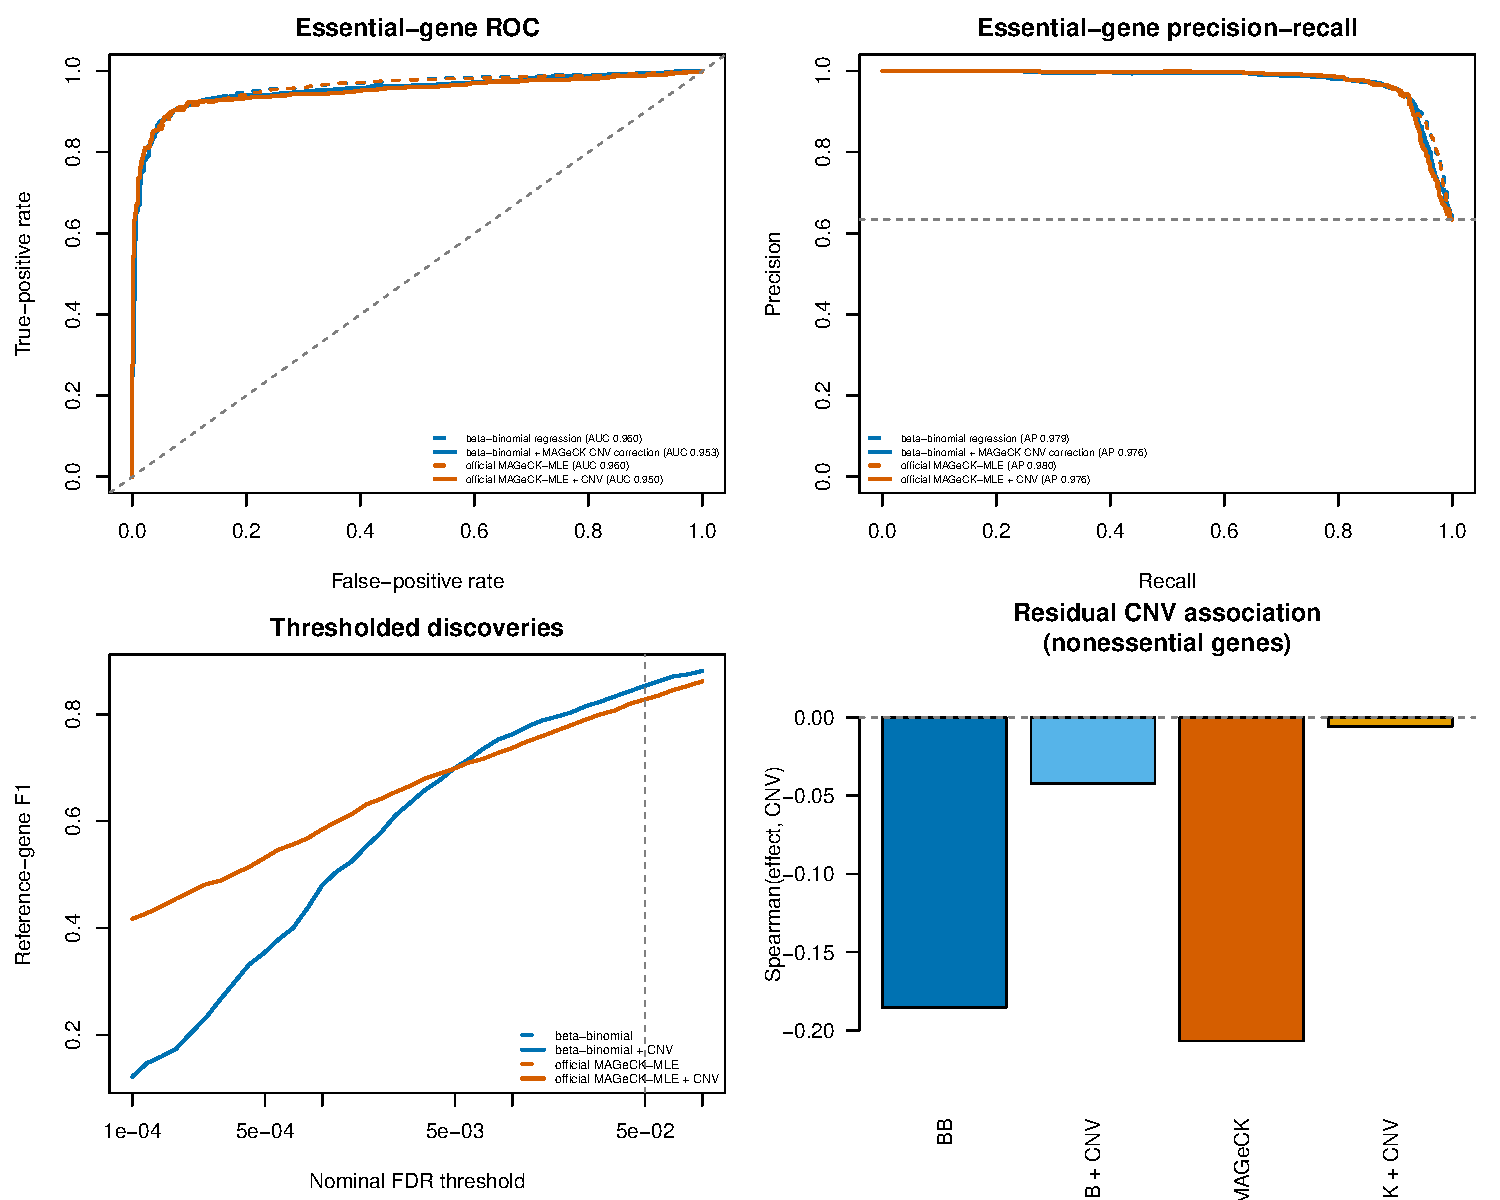
\includegraphics[width=\textwidth]{figures/sanson_gold_standard_benchmark.pdf}
\caption{CNV-aware essential-gene discrimination in the Sanson A375 screen.
(A) ROC, (B) precision--recall, (C) F1 across nominal FDR thresholds, and
(D) absolute residual effect--CNV correlation among nonessential genes, where
values closer to zero are better.  Curves compare uncorrected (dashed) and
CNV-corrected (solid) BARCS and official MAGeCK-MLE results; open points mark
CNV-corrected values.}
\label{fig:sanson}
\end{figure}

\subsection{External false-discovery benchmark: sensitivity to the analysis contract}

A recent Chronos hit-calling preprint compared CB\textsuperscript{2},
MAGeCK, JACKS, DrugZ, and Chronos on single-condition dependency calling and
differential viability \citep{dempster2025fdr}.  The deposited notebooks and
intermediate files make this comparison unusually auditable
\citep{dempster2025fdrdata}.  They expose two distinct observations that
should not be conflated.  Original CB\textsuperscript{2} has a genuine
small-sample power limitation in two-versus-two condition comparisons, but
the strongest reported evidence of anti-conservative CB\textsuperscript{2}
inference is sensitive to an incompatible preprocessing step.

For guide $g$ and sample $j$, CB\textsuperscript{2} constructs the library
total internally as
\[
N_j=\sum_{g\in\mathcal{G}}K_{gj}.
\]
The null-only Avana benchmark first restricted the count matrix to selected
control genes and then ran CB\textsuperscript{2}.  Consequently, its
beta-binomial denominator became
\[
N_j^{\mathrm{subset}}
  =\sum_{g\in\mathcal{G}_{0}}K_{gj},
\]
rather than the full sequencing depth.  Filtering guides is legitimate for
evaluation, but it must occur after fitting or be accompanied by immutable
full-library totals.  This distinction matters because within-sample
rescaling leaves guide proportions unchanged while changing the
beta-binomial sampling variance through $N_j$.

We audited this point using the deposited \texttt{CB2\_no\_positives.csv} and
\texttt{CB2\_allgenes.csv} files.  The published subset-matrix analysis
reports 152 test-negative discoveries at FDR 0.1.  Restricting the
full-library CB\textsuperscript{2} $p$-values to exactly the same test genes
and reapplying Benjamini--Hochberg gives zero discoveries in all five cell
lines (Table~\ref{tab:chronosaudit}).  The nominal $p<0.05$ frequency still
reaches 14.5\% and 11.7\% in two lines, so this correction does not establish
perfect calibration.  It does show that the reported 152 discoveries are not
evidence about CB\textsuperscript{2} fitted with its required full-library
denominator.  A second concern is that the common preprocessing applies
Chronos negative-control normalization and rounding before all fits.  That
transformation is meaningful for Chronos, but it changes the effective
sequencing depths of a method whose likelihood treats read totals as sampling
information.  Equal preprocessing is therefore not automatically equivalent
to equal model input.

\begin{table}[ht]
\centering
\caption{Audit of the version-1 Chronos false-discovery benchmark.  The
Avana row uses the same test genes under two library-total contracts.  The
PSN1 and DeWeirdt rows are direct BARCS reruns on the
deposited normalized count tables; ``known'' denotes the 28 literature-curated
condition--gene combinations used by the preprint, not a complete truth set.}
\label{tab:chronosaudit}
\small
\setlength{\tabcolsep}{5pt}
\begin{tabular}{p{0.31\textwidth}p{0.27\textwidth}p{0.31\textwidth}}
\toprule
Audit target & \methodswatch{cbtwocyan} Reported legacy result &
\methodswatch{barcsblue} BARCS reanalysis\\
\midrule
Avana null-only, FDR $<0.1$ &
152 false discoveries after pre-fit guide subsetting &
0 after preserving full-library totals\\
PSN1 two-versus-two null split &
0 gene discoveries; conservative gene $p$-values &
4.81\% guide $p<0.05$, 4.65\% after control scaling, and 0 gene discoveries\\
DeWeirdt differential screens &
0 discoveries and 0/28 known interactions &
38 discoveries and 1/28 known interactions\\
\bottomrule
\end{tabular}
\end{table}

The differential-screen limitation is real.  Original
CB\textsuperscript{2} estimates each condition separately and uses the
Welch--Satterthwaite degrees of freedom
\[
\nu=
\frac{(\widehat V_A+\widehat V_B)^2}
{\widehat V_A^2/(n_A-1)+\widehat V_B^2/(n_B-1)}.
\]
With $n_A=n_B=2$, $1\leq\nu\leq2$.  Two independent variance estimates and a
heavy-tailed reference distribution leave little power.  In contrast,
BARCS estimates one guide-level dispersion across the full
design.  On the PSN1 pseudo-condition split, its guide-level null is close to
nominal and its negative-control scale is 1.017.  This is evidence that pooled
regression repairs part of the finite-sample problem.

It does not solve the full Chronos task.  In an exploratory rerun of the ten
DeWeirdt comparisons used for the curated-positive analysis
\citep{deweirdt2020isogenic}, BARCS used the four terminal
libraries, full count-table totals, a treatment coefficient, guide-level
control scaling, Fisher gene aggregation, and BH correction.  It recovered
MCL1 under A-1331852 in Meljuso, but only one of 28 curated interactions
overall.  Thirty-seven of its 38 discoveries came from OVCAR8 under olaparib,
without recovering BRCA1 or BRCA2.  This pattern is consistent with a global
difference in screen sensitivity rather than a failure that one additional
fixed covariate can remove: with two replicates per arm, a treatment-associated
quality shift is nearly collinear with treatment itself.  Negative controls
that are inactive in both arms also need not represent artifacts affecting
strong common-essential knockouts.

The version-1 notebook raises two further reproducibility issues.  First, its
FDR-calibration helper accepts a requested evaluation gene set but does not
use that argument; the calibration curve therefore includes training controls
used by Chronos as well as held-out controls.  Second, calls intended to remove
MAGeCK's \texttt{common} coefficient use a non-mutating
\texttt{DataFrame.drop()} without assigning the returned object.  In the PSN1
calibration, this leaves 34,124 MAGeCK entries versus 17,787 entries for
CB\textsuperscript{2}, JACKS, DrugZ, and Chronos.  These implementation details
do not invalidate the biological motivation for empirical-null hit calling,
but they make the strongest method-ranking and calibration claims provisional.
Similarly, treating thousands of correlated gene--screen indicators as
independent observations in a $t$ test yields uncertainty that is narrower
than a screen- or cell-line-clustered bootstrap would provide.

The appropriate conclusion is therefore narrower than either ``CB\textsuperscript{2}
is miscalibrated'' or ``BARCS solves false discovery.''
The regression extension repairs the mean-model and dispersion-pooling
limitations, accepts CNV and other identifiable sample covariates, and gives a
well-behaved null in the PSN1 check.  It does not by itself supply Chronos's
growth dynamics, replicate-quality terms, or empirical differential null.
A production differential-screen method still needs immutable library totals,
raw-count or likelihood-compatible normalization, dispersion moderation,
correlation-aware gene aggregation, held-out control calibration, and blocked
replicate-label permutations.
